\documentclass[10pt,letterpaper,spanish,numbers=endperiod]{article}
\usepackage[spanish]{babel}
\usepackage[ansinew]{inputenc}
\usepackage[right=2cm,left=0.5cm,top=0cm,bottom=2cm,headsep=0cm,footskip=0.5cm]{geometry}
%\usepackage[dvips]{graphicx}
\usepackage{graphicx}
\usepackage{wrapfig}
\usepackage{ragged2e}
\usepackage[table]{xcolor}
\usepackage{color, colortbl}
\usepackage{hhline}
\usepackage{tabularx,colortbl}
\usepackage{tikz}
\usepackage{enumerate}

%Ruta de las imagenes
\graphicspath{ {./imgs/} }

% Mejora la cinfiguracion de las secciones
\usepackage[colorlinks]{hyperref} 
\usepackage{cleveref}
\makeatletter
\def\@seccntformat#1{\@ifundefined{#1@cntformat}%
   {\csname the#1\endcsname\space}    
   {\csname #1@cntformat\endcsname}}% habilita el control individual
\newcommand\section@cntformat{\thesection.\space}       % Nivel Section
\newcommand\subsection@cntformat{\thesubsection.\space} % Nivel de Subsection
\makeatother

\usepackage{xparse}
\NewDocumentCommand{\Contenido}{mmm}
 {
  \subsection{#1} \label{sec:#2}
	\centerline{\begin{minipage}{.4\textwidth}
		\includegraphics[width=\linewidth, height=60mm]{#3}
	\end{minipage}}
 }

\begin{document}

%Comandos para el diseño del documento
\newcommand{\linea} %Agregamos una linea
    {
    \vskip 0.5cm
    }
		
\newcommand{\lineas} %Agregamos una linea mas ancha
    {
    \vskip 2cm
    }
\newcommand{\masLineas} %Agregamos una linea mas ancha
    {
    \vskip 8cm
    }		

\newcommand{\nuevaPagina} %Agregamos una linea mas ancha
	{		
			\pagebreak  %Salto a pagina 2 y encabezados
			\noindent\begin{minipage}{0.2\textwidth} %logo
			
\includegraphics[width=\linewidth]{logo2}
			\end{minipage}
	}
	
\newenvironment{centrar}{% Permite centrar un bloque de texto
  \setlength\topsep{0pt}
  \setlength\parskip{0pt}
  \begin{center}
}{\end{center}}
		
		
\noindent\begin{minipage}{0.2\textwidth}

\includegraphics[width=\linewidth]{logo}
\end{minipage}

\masLineas

%pintamos una linea roja
\begin{tikzpicture}[ultra thick]
\draw[red,thick] (0,0) -- (\textwidth,0);
\end{tikzpicture}

\linea
\begin{centrar}
Taller de Dise\~no de Aplicaciones
\end{centrar}
\linea

%pintamos una linea roja
\begin{tikzpicture}[ultra thick]
\draw[red,thick] (0,0) -- (\textwidth,0);
\end{tikzpicture}


\nuevaPagina

\large\bfseries Configuraci\'on de equipamiento y de red para Teletrabajo en empresa FastDevelopment
\linea
\textbf{Pasos para la configuraci\'on del servidor:}
\normalsize 
\linea
\section{Configuraci\'on de arranque} \label{sec:uno}

\centerline{\begin{minipage}{0.8\textwidth}
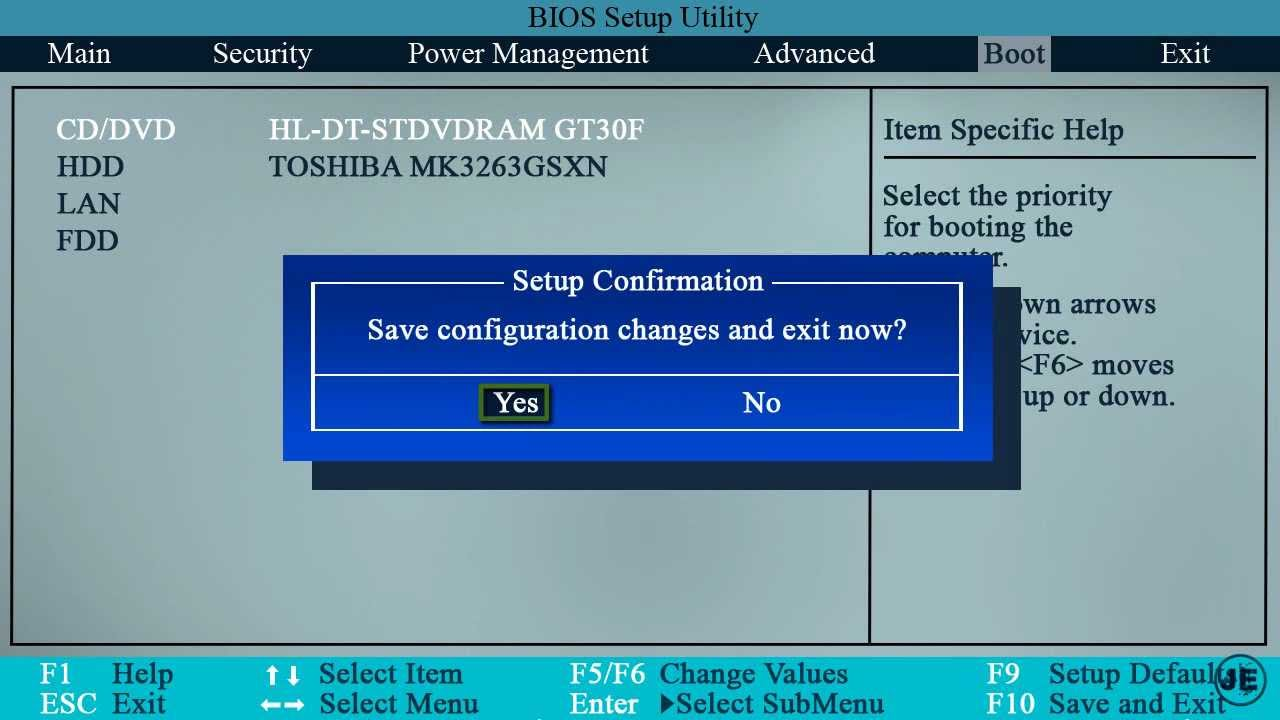
\includegraphics[width=\linewidth]{arranque}
\end{minipage}}
\linea
\subsection{Reiniciar el equipo} \label{sec:uno_uno}
\subsection{Presionar  la tecla asociada para acceder al men\'u de configuraci\'on de la BIOS. Normalmente suele ser Delete (Supr) o F2 pero dependiendo del fabricante de la misma tambi\'en pudiera ser F1, F10, F11, F12.} \label{sec:uno_dos}
\subsection{Desplazarse por los distintos men\'us de la BIOS hasta localizar Advanced BIOS Features (Caracter\'isticas avanzadas de la BIOS), dependiendo del fabricante. tambi\'en puede aparecer como Boot dentro del men\'u mostrado en la parte superior (seg\'un la imagen), o incluso alguna otra opci\'on diferente.} \label{sec:uno_tres}
\subsection{Modificar la opci\'on First Boot Device (Primer dispositivo de arranque) eligiendo seg\'un nuestras necesidades: CD, Floppy, USB (Remove device).} \label{sec:uno_cuatro}
\subsection{Salir y guardar los cambios. Esta opci\'on suele realizarse pulsando F10 (Save & Exit Setup) y luego confirmando la operaci\'on en el men\'u de confirmaci\'on.} \label{sec:uno_cinco}

\nuevaPagina

\section{Configuraci\'on del S.O.} \label{sec:dos}
Para esta implementaci\'on se ha seleccionado la distribuci\'on del Sistema Operativo Debian, sobre una maquina virtual Oracle VM.


\begin{table}[h!]
  \centering
  \begin{tabular}{c c}
    \begin{minipage}{.4\textwidth}
      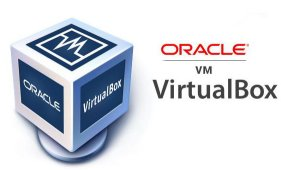
\includegraphics[width=\linewidth, height=60mm]{logoVirtualBox}
    \end{minipage}
    &
     \begin{minipage}{.3\textwidth}
      
\includegraphics[width=\linewidth, height=60mm]{debian_stretch}
    \end{minipage}
  \end{tabular}
\end{table}

\linea
\Contenido{Creaci\'on de maquina Servidor}{dos_uno}{paso_1}

\linea
\Contenido{Creaci\'on de disco duro (HDD)}{dos_dos}{paso_2}

\nuevaPagina
\linea

\linea
\Contenido{Se inserta ISO a unidad \'optica}{dos_tres}{paso_3}

\linea
\Contenido{Se habilita 1 tarjeta de red}{dos_cuatro}{paso_4}

\linea
\Contenido{Se habilita segunda tarjeta de red, en esta ocasi\'on de mantendr\'a como desconectada mientras se realiza la instalaci\'on del S.O.}{dos_cinco}{paso_5}

\nuevaPagina

\linea
\Contenido{Se Inicia MV usando el .ISO configurado inicialmente}{dos_sies}{paso_6}

\linea
\Contenido{Selecci\'on de idioma para el proceso de intalaci\'on}{dos_siete}{paso_7}

\linea
\Contenido{Selecci\'on de ubicaci\'on}{dos_ocho}{paso_8}

\nuevaPagina

\linea
\Contenido{Selecci\'on de la distribuci\'on del teclado}{dos_nueve}{paso_9}

\linea
\Contenido{Selecci\'on de tarjeta de red}{dos_diez}{paso_10}

\linea
\Contenido{Configuraci\'on del nombre maquina}{dos_once}{paso_11}

\nuevaPagina

\linea
\Contenido{Ingreso de nombre de dominio de Cliente}{dos_doce}{paso_12}

\linea
\Contenido{Configuraci\'on de Password Superusuario o ROOT}{dos_trece}{paso_13}

\linea
\Contenido{Introducimos nuevamente la contrase\~na para verificaci\'on}{dos_catorce}{paso_14}

\nuevaPagina

\linea
\Contenido{Cuenta de usuario administrador}{dos_quince}{paso_15}

\linea
\Contenido{Nombre de usuario}{dos_dieciseis}{paso_17}

\linea
\Contenido{Contrase\~na de la cuenta de usuario}{dos_dieciciete}{paso_18}

\nuevaPagina

\linea
\Contenido{Selecci\'on de zona horaria}{dos_dieciocho}{paso_19}

\linea
\Contenido{Seleccionamos el m\'etodo de la partici\'on manual}{dos_diecinueve}{paso_20}

\linea
\Contenido{Seleccionamos el disco a utilizar}{dos_veinte}{paso_21}

\nuevaPagina

\linea
\Contenido{Advertencia antes de crear la nueva tabla de particiones}{dos_veintiuno}{paso_22}

\linea
\Contenido{Podemos observar el espacio libre}{dos_veintidos}{paso_23}

\linea
\Contenido{Creamos una nueva partici\'on}{dos_veintitres}{paso_24}

\nuevaPagina

\linea
\Contenido{Especificamos el tama\~no de la SWAP, que dejaremos en 1GB}{dos_veinticuatro}{paso_25}

\linea
\Contenido{Seleccionamos el tipo de Partici\'on creada}{dos_veinticinco}{paso_26}

\linea
\Contenido{Seleccionamos Principio para continuar con la creaci\'on de las particiones}{dos_veintiseis}{paso_27}

\nuevaPagina

\linea
\Contenido{Podemos observar el resultado del proceso anterior}{dos_veinticiete}{paso_28}

\linea
\Contenido{Seleccionamos como se utilizara la partici\'on creada}{dos_veintiocho}{paso_29}

\linea
\Contenido{Se finaliza con la creaci\'on del \'area de intercambio}{dos_veintinueve}{paso_30}

\nuevaPagina

\linea
\Contenido{Continuamos, como en los pasos anteriores, con la creaci\'on de las particiones de /root (Donde se encuentra ubicado el directorio ra\'iz '/' con excepci\'on del /boot) y la partici\'on /home}{dos_treinta}{paso_31}

\linea
\Contenido{Las particiones fueron creadas y finalizamos con el particionado}{dos_treintaydos}{paso_32}

\linea
\Contenido{Despu\'es de confirmar la escritura del particionado, comienza la instalaci\'on}{dos_treintaytres}{paso_33}

\nuevaPagina

\linea
\Contenido{Durante la instalaci\'on se despliega la siguiente ventana para la configuraci\'on de los paquetes de Debian, donde debemos seleccionar 'No' porque no contamos con otro disco}{dos_treintaycuatro}{paso_34}

\linea
\Contenido{En la siguiente consulta, selecionamos 'No', para permitir una instalaci\'on reducida del S.O.}{dos_treintaycinco}{paso_35}

\linea
\Contenido{Configuramos el gestor de paquetes para que nuestra distribuci\'on se mantenga actualizada}{dos_treintayseis}{paso_36}

\nuevaPagina

\linea
\Contenido{Instalaci\'on del gestor de arranque multiple GRUB}{dos_treintayciete}{paso_37}

\linea
\Contenido{Selecci\'on de la ubicaci\'on del gestor de arranque GRUB}{dos_treintayocho}{paso_38}

\linea
\Contenido{Mensaje del t\'ermino de la Instlacion del S.O.}{dos_treintaynueve}{paso_39}

\nuevaPagina

\linea
\Contenido{Reinicio de la maquina y arranque del servidor}{dos_cuarenta}{paso_40}

\end{document}